%%%%%%%%%%%%%%%%%%%%%%%%%%%%%%%% COMMENT THIS TO COMPILE main.tex %%%%%%%%%%%%%%%%%%%%%%%%%%%%%%%%
\documentclass[a4paper,12pt]{report}
\usepackage[english]{babel}
\usepackage[left=2cm,right=2cm,top=2cm,bottom=2cm]{geometry}
%\usepackage{mathtools}
\usepackage{amsthm}     % for definitions and theorems
\usepackage[many]{tcolorbox}    % boxes around definitions and theorems
%\usepackage{amsmath}
%\usepackage{nccmath}
\usepackage{amssymb}    % \ltimes
\usepackage{etoolbox}   % for start of Chapter
%\usepackage{amsfonts}
\usepackage{physics}    % for all Physics related
\usepackage{dsfont}     % for the identity matrix symbol \1
%\usepackage{mathrsfs}

\usepackage{titling}
\usepackage{indentfirst}

\usepackage{bm}
\usepackage[dvipsnames]{xcolor}
\usepackage{cancel}

\usepackage{xurl}
\usepackage[colorlinks=true]{hyperref}

\usepackage{float}
\usepackage{graphicx}
\usepackage{subcaption}
%\usepackage{tikz}

\usepackage{ctable}     % tabelas
\renewcommand{\P}{\phantom{+}}  % empty space to indent things
\usepackage{multirow}
\usepackage{tabulary}

%%%%%%%%%%%%%%%%%%%%%%%%%%%%%%%%%%%%%%%%%%%%%%%%%%%

\newcommand{\eps}{\epsilon}
\newcommand{\vphi}{\varphi}
\newcommand{\cte}{\text{cte}}

\newcommand{\N}{{\mathbb{N}}}
\newcommand{\Z}{{\mathbb{Z}}}
%\newcommand{\Q}{{\mathbb{Q}}}
\newcommand{\C}{{\mathbb{C}}}
\renewcommand{\S}{{\hat{S}}}
%\renewcommand{\H}{\s{H}}

\renewcommand{\a}{{\vb{a}}}
\renewcommand{\b}{{\vb{b}}}
\renewcommand{\d}{{\dagger}}
\newcommand{\up}{{\uparrow}}
\newcommand{\down}{{\downarrow}}
\newcommand{\hc}{{\text{h.c.}}}

\newcommand{\ihat}{\bm{\hat{\imath}}}
\newcommand{\jhat}{\bm{\hat{\jmath}}}
\newcommand{\khat}{\bm{\hat{k}}}

\newcommand{\0}{{\vb{0}}}
\newcommand{\1}{\mathds{1}}
\newcommand{\E}{{\vb{E}}}
\newcommand{\B}{{\vb{B}}}
\renewcommand{\u}{{\vb{u}}}
\renewcommand{\v}{{\vb{v}}}
\renewcommand{\r}{{\vb{r}}}
\newcommand{\R}{{\vb{R}}}
\newcommand{\Q}{{\vb{Q}}}
\newcommand{\G}{{\vb{G}}}
\newcommand{\g}{{\vb{g}}}
\renewcommand{\k}{{\vb{k}}}
\newcommand{\K}{{\vb{K}}}
\newcommand{\p}{{\vb{p}}}
\newcommand{\q}{{\vb{q}}}
\newcommand{\F}{{\vb{F}}}
\renewcommand{\t}{{\vb{t}}}
\newcommand{\vtau}{{\bm{\tau}}}
\newcommand{\vdelta}{{\bm{\delta}}}

% COLORED SYMMETRY ELEMENTS
\newcommand{\Ct}{{\textcolor{Cyan}{C_3}}}
\newcommand{\Ctn}[1]{{\textcolor{Cyan}{C_3^{\textcolor{black}{#1}}}}}
\newcommand{\Cs}{{\textcolor{ForestGreen}{C_6}}}
\newcommand{\Csn}[1]{{\textcolor{ForestGreen}{C_6^{\textcolor{black}{#1}}}}}
\newcommand{\sd}{{\textcolor{RoyalBlue}{\sigma_d}}}
\newcommand{\sdn}[1]{{\textcolor{RoyalBlue}{\sigma_d^{\textcolor{black}{#1}}}}}
\newcommand{\sdp}{{\textcolor{RoyalBlue}{\sigma_d'}}}
\newcommand{\sdpp}{{\textcolor{RoyalBlue}{\sigma_d''}}}
\newcommand{\sv}{{\textcolor{Orange}{\sigma_v}}}
\newcommand{\svn}[1]{{\textcolor{Orange}{\sigma_v^{\textcolor{black}{#1}}}}}
\newcommand{\svp}{{\textcolor{Orange}{\sigma_v'}}}
\newcommand{\svpp}{{\textcolor{Orange}{\sigma_v''}}}

\newcommand{\s}{\sigma}
%\newcommand{\prodint}[2]{\left\langle #1 , #2 \right\rangle}
\newcommand{\cc}[1]{\overline{#1}}
\newcommand{\Eval}[3]{\eval{\left( #1 \right)}_{#2}^{#3}}
\newcommand{\sg}[2]{\{ #1 \mid #2 \}}

\newcommand{\unit}[1]{\; \mathrm{#1}}

\newcommand{\n}{\medskip}
\newcommand{\e}{\quad \mathrm{and} \quad}
\newcommand{\ou}{\quad \mathrm{or} \quad}
\newcommand{\virg}{\, , \;}
\newcommand{\ptodo}{\forall \,}
\renewcommand{\implies}{\; \Rightarrow \;}
%\newcommand{\eqname}[1]{\tag*{#1}} % Tag equation with name

\setlength{\droptitle}{-7em}

\makeatletter
\patchcmd{\chapter}{\if@openright\cleardoublepage\else\clearpage\fi}{}{}{}  % start 'Chapter' at the same page. needs package etoolbox
\makeatother

%% Theorems, definitions, proofs
\theoremstyle{definition}

\newtheorem{definition}{Definition}[section]
\tcolorboxenvironment{definition}{
  colback=blue!5!white,
  boxrule=0pt,
  boxsep=1pt,
  left=2pt,right=2pt,top=2pt,bottom=2pt,
  oversize=2pt,
  sharp corners,
  before skip=\topsep,
  after skip=\topsep,
}

\newtheorem{theorem}{Theorem}[section]
\tcolorboxenvironment{theorem}{
  colback=blue!5!white,
  boxrule=0pt,
  boxsep=1pt,
  left=2pt,right=2pt,top=2pt,bottom=2pt,
  oversize=2pt,
  sharp corners,
  before skip=\topsep,
  after skip=\topsep,
}

\begin{document}
%%%%%%%%%%%%%%%%%%%%%%%%%%%%%%%% COMMENT THIS TO COMPILE main.tex %%%%%%%%%%%%%%%%%%%%%%%%%%%%%%%%

%%%%%%%%%%%%%%%%%%%%%%%%%%%%%%%%%%%%%%%%%%%%%%%%%%%%%%%%%%%%%%%%%%%%%%%%%%%%%%%%%%%%%%%%%%%%%%%%%%
\chapter{Groups and Representations} \label{ch:group_theory}
%%%%%%%%%%%%%%%%%%%%%%%%%%%%%%%%%%%%%%%%%%%%%%%%%%%%%%%%%%%%%%%%%%%%%%%%%%%%%%%%%%%%%%%%%%%%%%%%%%

\textbf{TODO:}
\begin{itemize}
\item \textbf{ENUMERAR EQUAÇÕES.}
\item \textbf{MELHORAR O TEXTO DAS CAPTIONS.}
\item \textbf{MELHORAR A INTRODUÇÃO/MOTIVAÇÃO.}
\item \textbf{ESCREVER SOBRE INDUCTION/SUBDUCTION}
\item \textbf{ESCREVER SOBRE SPACE GROUPS}
\item \textbf{ESCREVER SOBRE MAGNETIC SPACE GROUPS}
\end{itemize}

The concept of \textit{symmetry} reincidentally appears in physics, because various aspects of our reality exhibit symmetric objects.

Our goal is to develop a fully symmetric model for TBG. To achieve this, it is essential to first understand the mathematical concepts of symmetry, specifically Group Theory and Representation Theory as applied to crystallographic solids. In this chapter we will provide the necessary definitions and theorems in order to develop our symmetry analysis.

%%%%%%%%%%%%%%%%%%%%%%%%%%%%%%%%%%%%%%%%%%%%%%%%%%%%%%%%%%%%%%%%%%%%%%%%%%%%%%%%%%%%%%%%%%%%%%%%%%
\section{Group theoretic concepts} \label{sec:group_theoretic_concepts}
%%%%%%%%%%%%%%%%%%%%%%%%%%%%%%%%%%%%%%%%%%%%%%%%%%%%%%%%%%%%%%%%%%%%%%%%%%%%%%%%%%%%%%%%%%%%%%%%%%

In this thesis we are concerned with symmetries that relate to graphene. Because its carbon atoms form a honeycomb lattice, our basic object of study will be a 2D hexagon.

\begin{figure}[H]
\centering
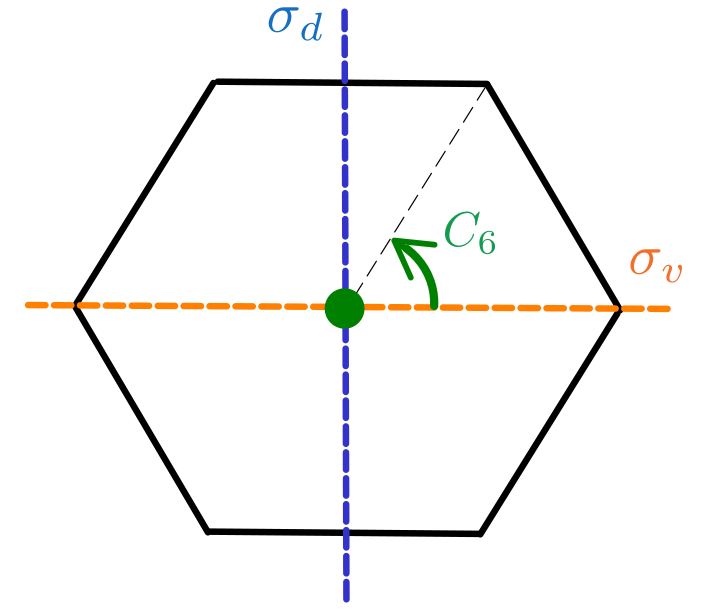
\includegraphics[width=0.4\linewidth]{fig/hexagon.png}
\caption{2D spatial symmetries of a hexagon.}
\label{fig:hexagon}
\end{figure}

\begin{example} \label{ex:symm_elems_hexagon_D6_example}
In a certain sense, a basic hexagon has 12 symmetry elements. Looking at Figure \ref{fig:hexagon}, the hexagon has the reflections $\sd$, $\sv$, the $60^\circ$ rotation $\Cs$, and all the combinations of these. Combining all the possibilities, we say all that the symmetry elements of the hexagon form the \textit{group}
\begin{equation} \label{eq:all_D6_elements}
D_6 = \{E, \Cs, \underbrace{\Ct}_{\Csn{2}}, \underbrace{C_2}_{\Csn{3}}, \underbrace{\Ctn{2}}_{\Csn{4}}, \Csn{5}, \sd, \underbrace{\sdp}_{\sd \Ct}, \underbrace{\sdpp}_{\sd \Ctn{2}}, \sv, \underbrace{\svp}_{\sv \Ct}, \underbrace{\svpp}_{\sv \Ctn{2}} \}.
\end{equation}
In this list, we did not include repeated elements, observe that $\Csn{6} = \sdn{2} = \svn{2} = E$ is the element the identity element, the one that ``does nothing''.
\end{example}


The concept of \textit{group} $G$ grasps the set of elements $a \in G$ that represent the symmetry of an object, along with its symmetry operation ``$\vdot$''. The element $a \vdot b$ represents the ``composition'' of applying first the operation $a$, and then $b$.

\begin{definition}[\textbf{Group}] \label{def:group}
Given a set $G$ and a binary operation ``$\vdot$''$:G\times G \to G$, \textbf{the pair} $(G, \vdot)$ is called a \textit{group} if it satisfies the following properties:
\begin{enumerate}
\item (closure): $a \vdot b \in G$, for every $a, b \in G$.
\item (associativity): $(a \vdot b) \vdot c =  a \vdot (b \vdot c)$, for every $a, b, c \in G$.
\item (identity): There exists an (identity) element $E \in G$ such that $E \vdot a = a \vdot E = a$, for every $a \in G$.
\item (inverse): For every $a \in G$, there is (an inverse) $a^{-1} \in G$ such that $a \vdot a^{-1} = a^{-1} \vdot a = E$.
\end{enumerate}
\end{definition}
Normally in the literature, one speaks of the set $G$ as being ``the group'' instead of the pair $(G, \vdot)$ and omits the operation symbol ``$\vdot$'', simply writing $ab$ instead of $a \vdot b$. This is for convenience but, mathematically, the operation ``$\vdot$'' is crucial to define a group.

\begin{definition}[\textbf{Order}] \label{def:group_order}
Given any set $A$, we denote its number of elements by $\abs{A}$. The \textit{order} of a group $G$ is defined simply as its number of elements $\abs{G}$.
\end{definition}

\begin{example} \label{ex:subgroup_example_D3D6}
Frequently, an object $A$ has all the symmetries of another object $B$. In Figure \ref{fig:hexagon_subgroup}, the \textcolor{ForestGreen}{green hexagon} has all the symmetries of the \textcolor{Cyan}{cyan triangle}. The symmetry elements of the triangle form the group $D_3 = \{E, \Ct, \Ctn{2}, \sv, \svp, \svpp\}$. Because $D_3$ is a subset of $D_6$ and also forms a group by itself, we say that $D_3$ is a subgroup of $D_6$.
\end{example}

\begin{figure}[H]
\centering
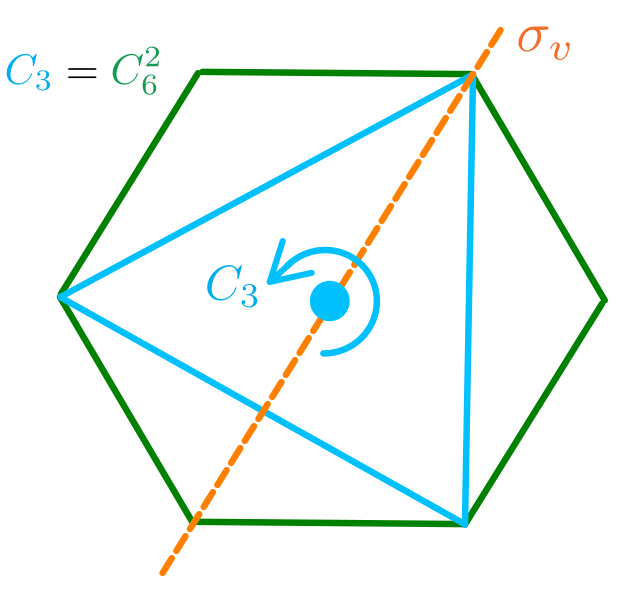
\includegraphics[width=0.4\linewidth]{fig/hexagon_subgroup.png}
\caption{The \textcolor{ForestGreen}{hexagon} has all the symmetries of the \textcolor{Cyan}{triangle}, i.e., $D_3$ is a subgroup of $D_6$.}
\label{fig:hexagon_subgroup}
\end{figure}


\begin{definition}[\textbf{Subgroup}] \label{def:subgroup}
If $(G, \vdot)$ is a group and $H$ is a subset of $G$, we say that $H$ is a subgroup of $G$ if the pair $(H, \vdot)$ is a group by itself.
\end{definition}

It is common that one defines a group by its \textit{generators}. We did that when defining the groups $D_6$ and $D_3$ associated to the hexagon and triangle, respectively at Figures \ref{fig:hexagon} and \ref{fig:hexagon_subgroup}. By generators, we mean:

\begin{definition}[\textbf{Generators of a group}] \label{def:generators_of_group}
If $S$ is a subset of a group $G$, we define $\ev{S}$ as the smallest subgroup of $G$ containing every element of $S$. The subgroup $\ev{S}$ is called the \textit{subgroup generated by $S$}. If $\ev{S} = G$, we say that the set $S$ \textit{generates} $G$.
\end{definition}


\begin{example} \label{ex:generators_example}
An intuitive way of thinking of $\ev{S}$ is by ``recursively multiplying'' all the elements of $S$, until all the possibilities are exhausted. In general for two elements:
\begin{equation} \label{eq:generate_two_elements}
\ev{\{a,b\}} = \{E, a, b, a^2, ab, ba, b^2, a^3, a^2b, aba, ba^2, ab^2, bab, b^2a, b^3, \ldots\}.
\end{equation}

For the hexagon at Figure \ref{fig:hexagon}, the set $\{\Cs, \sd, \sv\}$ generates the group $D_6$; and for the triangle at Figure \ref{fig:hexagon_subgroup}, the set $\{\Ct, \sv\}$ generates the group $D_3$.
\end{example}


\begin{definition}[\textbf{Cosets}] \label{def:left_cosets}
Let $G$ be a group and $H$ one of its subgroups. Given an element $g \in G$, we define the set $gH$ by
\begin{equation} \label{eq:gH_left_coset}
gH = \{g h \mid h \in H\} \subseteq G.
\end{equation}
This set $gH$ is called a \textit{left coset} of $G$ with respect to $H$, and $g$ is a \textit{representative} of $gH$. We denote the set of left cosets of $H$ by
\begin{equation} \label{eq:G/H_left_cosets}
G/H = \qty{gH \subseteq G \mid g \in G}.
\end{equation}

It is always possible to decompose $G$ as a disjoint union of its left cosets:
\begin{equation} \label{eq:disjoint_union_leftcosets}
G = \bigcup_{j=1}^{\abs{G/H}} g_j H = \sum_{j=1}^{\abs{G/H}} g_j H,
\end{equation}
where $g_j \in G$ is a representative of $g_j H$, and $\abs{G/H}$ is the number of different left cosets.
\end{definition}

An iconic theorem due to Laplace says that the order of a subgroup $H \subseteq G$ divides the order of the group $G$.

\begin{theorem}[\textbf{Laplace}]
The number of different left cosets is given by $\abs{G/H} = \abs{G} / \abs{H}$.
\end{theorem}

\begin{example} \label{ex:coset_decomp_D3D6}
As an example, take $H = D_3$ and $G = D_6$. We have that $\abs{D_3}=6$ and $\abs{D_6} = 12$. Therefore, we only have two different left cosets. One of them has $E$ as its representative:
\begin{equation} \label{eq:ED3-D6-first_coset}
E D_3 = D_3 = D_3 = \{E, \Ct, \Ctn{2}, \sv, \svp, \svpp\}.
\end{equation}

The other one is what is left of $D_6$, which has $\sd$ as its representative:
\begin{equation} \label{eq:sdD3-D6-second_coset}
\sd D_3 = \{\sd E, \sd \Ct, \sd \Ctn{2}, \sd \sv, \sd \svp, \sd \svpp\}
= \{ \sd, \sdp, \sdpp, C_2, \Csn{5}, \Cs \},
\end{equation}

The coset decomposition is the disjoint union of the two cosets
\begin{equation} \label{eq:D6_coset_decomp}
D_6 = ED_3 \cup \sd D_3.
\end{equation}
\end{example}

One would probably notice that the elements $\sd, \sdp, \sdpp$ are in some way related, also as $\sv, \svp, \svpp$. Actually, they belong to the same conjugacy class, which is a concept analogous to the notion of matrix similarity in Linear Algebra.

\begin{definition}[\textbf{Conjugacy classes}] \label{def:conj_class}
Let $G$ be a group and $a, g, g' \in G$. If $g' = a g a^{-1}$, we say that $g'$ is the \textit{conjugate} element of $g$ by means of $a$, and we write $g' \sim g$. The set
\begin{equation} \label{eq:defi_conjclass_[g]}
[g] = \{ g' \in G \mid g' \sim g \} = \{ a g a^{-1} \mid a \in G \} \subseteq G
\end{equation}
is called a \textit{conjugacy class} of $G$. Every group is a disjoint union of its conjugacy classes.
\end{definition}

\begin{example} \label{ex:conjclass_example_D3D6}
For the groups $D_3$ and $D_6$, one finds the conjugacy classes

\begin{equation} \label{eq:D3_classes}
D_3 = [E] \cup [\Ct] \cup [\sv] = \{E\} \cup \{\Ct, \Ctn{2}\} \cup \{\sv, \svp, \svpp\},
\end{equation}
\begin{align} \label{eq:D6_classes}
D_6 &= \{E\} &&\cup&& \{C_2\} &&\cup&& \{\Ct, \Ctn{2}\} &&\cup&& \{\Cs, \Csn{5}\} &&\cup&& \{\sv, \svp, \svpp\} &&\cup&& \{\sd, \sdp, \sdpp\}.
\end{align}
\end{example}

\begin{example} \label{ex:homomorphism_sublattice_AB_example}
Let us say we want to identify which elements of $D_6$ exchange sublattice types $A$ and $B$, as in Figure \ref{fig:hexagon_AB}. We can accomplish this task by using a labelling function $\vphi: D_6 \to \{1, -1\}$, where
\begin{align} \label{eq:homomorphism_example_sublattices_AB_D6}
\vphi(g) =
\begin{cases}
\; \P1, \quad g \text{ changes sublattice type } A \leftrightarrow B, \\
\; -1, \quad \text{otherwise.}
\end{cases}
\end{align}

For our generators of $D_6$ we have $\vphi(\Cs) = -1$, $\vphi(\sv) = 1$ and $\vphi(\sd) = -1$. Only these values are sufficient, because if we treat $\{1, -1\}$ as a group by itself, with standard multiplication as its operation, one may notice that $\vphi$ follows the rule
\begin{equation} \label{eq:vphi_g1g2_homomophism}
\vphi(g_1 g_2) = \vphi(g_1) \vphi(g_2).
\end{equation}

The element $g_1 g_2$ changes sublattice only if exactly one of $g_1$ or $g_2$ do. Now, the elements $D_3$ do not exchange sublattice type, which translates to the property $\vphi(g) = 1$ for every $g \in D_3$.
\end{example}

\begin{figure}[H]
\centering
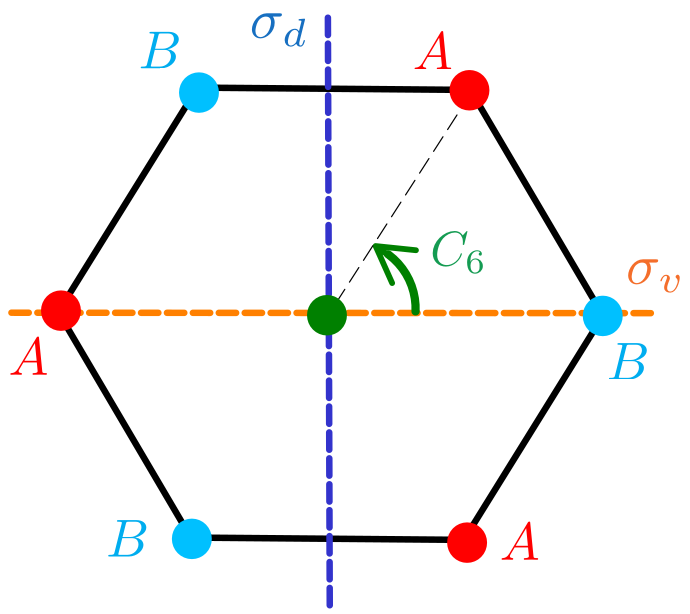
\includegraphics[width=0.4\linewidth]{fig/hexagon_AB.png}
\caption{Symmetries $D_6$ with sublattice type $A$ or $B$.}
\label{fig:hexagon_AB}
\end{figure}



The function $\vphi$ is generally known as a homomorphism, which in the case above identifies the subgroup $D_3$ as its kernel.

\begin{definition}[\textbf{Homomorphism}] \label{def:homomorphism}
Let $G$ and ${G'}$ be groups. A function $\vphi: G \to {G'}$ is called an \textit{homomorphism} if it preserves the group structure, i.e.,
\begin{equation} \label{eq:homomorphism}
\vphi(a b) = \vphi(a) \vphi(b), \quad \forall \, a,b \in G.
\end{equation}
If $\vphi$ is bijective, we also call it an \textit{isomorphism}. The kernel of $\vphi$ is defined as the set
\begin{equation} \label{eq:kernel_homomorphism}
\ker(\vphi) = \qty{g \in G \mid \vphi(g) = e_{G'}},
\end{equation}
where $e_{G'}$ is the identity element of ${G'}$.
\end{definition}

%%%%%%%%%%%%%%%%%%%%%%%%%%%%%%%%%%%%%%%%%%%%%%%%%%%%%%%%%%%%%%%%%%%%%%%%%%%%%%%%%%%%%%%%%%%%%%%%%%
\section{Elements of Representation Theory} \label{sec:representation_theory}
%%%%%%%%%%%%%%%%%%%%%%%%%%%%%%%%%%%%%%%%%%%%%%%%%%%%%%%%%%%%%%%%%%%%%%%%%%%%%%%%%%%%%%%%%%%%%%%%%%

In physics, specially in Quantum Mechanics, it is most common that one works with groups of matrices, where all the useful theorems of Functional Analysis hold.

\begin{definition}[\textbf{Groups of matrices}] \label{def:groups_of_matrices}
The set of invertible linear operators of a vector space $V$ form a group and we call it the \textit{general linear group}
\begin{equation} \label{eq:general_linear_GL(V)}
\GL(V) = \qty{A: V \to V \mid A \text{ is linear and invertible}}.
\end{equation}
If $V$ is finite dimensional with a scalar product, the set of unitary operators of $V$ is a subgroup of $\GL(V)$, defined by
\begin{equation} \label{eq:unitary_operators_U(V)}
\U(V) = \qty{A \in \GL(V) \mid A A^\dagger = \1}.
\end{equation}
%When $V = \mathbb{R}^n$ or $\C^n$, we can choose a basis and explicitly say that
%\begin{equation} \label{eq:GL(n)_defi}
%\GL(n, \mathbb{R}) = \qty{\text{invertible } n\times n \text{ real matrices}}, \;
%\GL(n, \mathbb{C}) = \qty{\text{invertible } n\times n \text{ complex matrices}}.
%\end{equation}
%In this case, the subgroups of orthogonal and unitary matrices are, respectively,
%\begin{equation} \label{eq:O(n)_defi}
%O(n) = \qty{A \in \GL(n, \mathbb{R}) \mid A A^T = \1}, \quad SO(n) = \qty{A \in O(n) \mid \det A = 1};
%\end{equation}
%\begin{equation} \label{eq:U(n)_defi}
%\U(n) = \qty{A \in \GL(n, \mathbb{C}) \mid A A^\dagger = \1}, \quad S\U(n) = \qty{A \in \U(n) \mid \det A = 1}.
%\end{equation}
\end{definition}

\begin{example} \label{ex:2x2_rep}
A group of $2\times 2$ matrices isomorphic to $D_3$ can be found by defining the homomorphism (representation) $\Gamma_2$ below
\begin{equation} \label{eq:D6_generators_2x2matrices}
\Gamma_2(\Ct) =
\begin{pmatrix}
\cos(\frac{2\pi}{3}) & \sin(\frac{2\pi}{3}) \\
-\sin(\frac{2\pi}{3}) & \cos(\frac{2\pi}{3})
\end{pmatrix},
\quad
\Gamma_2(\sd) =
\begin{pmatrix}
-1 & 0 \\
0 & 1
\end{pmatrix},
\quad
\Gamma_2(\sv) =
\begin{pmatrix}
1 & 0 \\
0 & -1
\end{pmatrix}.
\end{equation}

Imposing the homomorphism relation \ref{eq:homomorphism}, we can find all the representative $2\times 2$ matrices of $D_3$ by multiplying the matrices of the three generators in Equation \ref{eq:D6_generators_2x2matrices}.
\end{example}

\begin{definition}[\textbf{Representation}] \label{def:representation}
A \textit{representation} of a group $G$ on a vector space $V$ is a \textbf{homomorphism} $\Pi: G \to \GL(V)$.
\end{definition}

When applying the theory of representations to Quantum Mechanics, two key physical considerations must be incorporated. The first is the ability to change coordinate systems, and the second is the requirement to preserve probabilities by ensuring the unitarity of transformations.

\n

1. Conjugating an observable $H$ by means of $A$, as in $H' = A H A^{-1}$, corresponds to a change of reference frame (or basis). This leads us to regard two conjugate representations as equivalent, as they describe the same transformation in different bases.

\begin{definition}[\textbf{Equivalent representations}] \label{def:equiv_representations}
Two representations $\Pi_1: G \to \GL(V_1)$ and $\Pi_2: G \to \GL(V_2)$ of a group $G$ are said to be \textit{equivalent} if there is an invertible linear operator $A: V_1 \to V_2$ such that
\begin{equation} \label{eq:intertwiner}
\Pi_2(g) = A \Pi_1(g) A^{-1}, \, \forall \, g \in G.
\end{equation}
In this case we write $\Pi_1 \equiv \Pi_2$.
\end{definition}

2. In Quantum Mechanics, unitary matrices are standard because they preserve probabilities and ensure the physical consistency of the theory. Moreover, as we will see in Section \ref{sec:characters}, unitary representations are particularly significant due to the orthogonality theorems for representation characters, which fundamentally depend on this restriction. Lastly, this preference for unitary representations is not merely practical but is underpinned by the general principle stated in Theorem \ref{th:unitarity_rep} \cite{dresselhaus}.

\begin{theorem}[\textbf{Unitarity of representations}] \label{th:unitarity_rep}
A representation $\Gamma: G \to \GL(V)$ is called \textit{unitary} if $\Gamma(g) \in \U(V)$, $\forall \, g \in G$. Every representation $\Pi: G \to \GL(V)$ is equivalent to some unitary representation $\Gamma: G \to \U(V)$.
\end{theorem}

Because of Theorem \ref{th:unitarity_rep}, most of our theory will be dedicated to unitary representations. If not otherwise stated, when we consider a representation we actually mean an \textbf{unitary representation}.

\begin{example} \label{ex:direct_sum}
Considering $G = D_3$, take $\Gamma_2$ acting on $V_2 = \mathbb{R}^2$, as previously defined in Example \ref{ex:2x2_rep}, and also consider the trivial representation $\Gamma_1$ acting on $V_1 = \mathbb{R}$, which is defined by $\Gamma_1(g) = 1$, $\forall \, g \in G$. We can stack $\Gamma_2$ and $\Gamma_1$ to construct another representation $\Gamma$, acting on $V_2 \oplus V_1$, given by
\begin{equation} \label{eq:block_diagonal_Gamma_2_1}
\Gamma(g) =
\begin{pmatrix}
\Gamma_2(g) & 0 \\
0 & \Gamma_1(g)
\end{pmatrix}, \quad \forall \, g \in G.
\end{equation}
\begin{equation} \label{eq:D6_generators_3x3matrices}
\Gamma(\Ct) =
\begin{pmatrix}
\cos(\frac{2\pi}{3}) & \sin(\frac{2\pi}{3}) & 0 \\
-\sin(\frac{2\pi}{3}) & \cos(\frac{2\pi}{3}) & 0 \\
0 & 0 & 1
\end{pmatrix},
\;
\Gamma(\sd) =
\begin{pmatrix}
-1 & 0 & 0 \\
0 & 1 & 0 \\
0 & 0 & 1
\end{pmatrix},
\;
\Gamma(\sv) =
\begin{pmatrix}
1 & 0 & 0 \\
0 & -1 & 0 \\
0 & 0 & 1
\end{pmatrix}.
\end{equation}

We say that $\Gamma$ is a direct sum and we write $\Gamma \equiv \Gamma_2 \oplus \Gamma_1$. Representations, such as $\Gamma$, that can be decomposed into a direct sum are called \textit{reducible}. What distinguishes reducible representations is the existence of nontrivial invariant subspaces.
\end{example}

\begin{definition}[\textbf{Invariant subspace}] \label{def:invariant_subspace}
A vector subspace $W \subseteq V$ is said to be \textit{invariant} under a representation $\Pi: G \to \GL(V)$ if it satisfies $\Pi(g) W \subseteq W$ (the action of $\Pi(g)$ on $W$ is contained within $W$), for every $g \in G$.
\end{definition}

\begin{example} \label{ex:invariant_subspaces}
The nontrivial subspaces $V_2$ and $V_1$ are invariant under the action of $\Gamma$, defined in Example \ref{ex:direct_sum}. In Equation \ref{eq:block_diagonal_Gamma_2_1}, we see that $\Gamma(g)$ is block diagonal on subspaces $V_2$ and $V_1$, therefore we have that $\Gamma(g) V_2 \subseteq V_2$ and $\Gamma(g) V_1 \subseteq V_1$.
\end{example}

\begin{definition}[\textbf{Irreducible representation}] \label{def:irrep}
A representation $\Pi: G \to \GL(V)$ always has the trivial invariant subspace $\{0\}$ and $V$. If there are not others, $\Pi$ is said to be \textit{irreducible}.
\end{definition}

\begin{example} \label{ex:irrep_Gamma12_example}
Still in the context of Example \ref{ex:direct_sum}, unlike $\Gamma$, the representations $\Gamma_1$ and $\Gamma_2$ are \textit{irreducible} because they have no trivial invariant subspaces and are not equivalent to any block diagonal representation.
\end{example}

Theorem \ref{th:irreps_decomp}, whose proof can be found in \cite{dresselhaus, hamermesh}, states that irreducible representations (irreps) are building blocks for all representations in finite dimensional vector spaces.

\begin{theorem}[\textbf{Decomposition of unitary representations}] \label{th:irreps_decomp}
Let $V$ be a finite dimensional vector space with a scalar product and let $\Gamma: G \to \U(V)$ be an unitary representation. Then, $\Gamma$ is either irreducible or reducible and can be decomposed into a direct sum
\begin{equation} \label{eq:decomp_unitary_reps}
V = \bigoplus_{j=1}^N V_j, \quad
\Gamma(g) =
\begin{pmatrix}
\Gamma_1(g) &  &  \\
 & \ddots &  \\
 &  & \Gamma_N(g) \\
\end{pmatrix},
\end{equation}
where each $V_j$ is a nontrivial invariant subspace under $\Gamma$ and $\Gamma_j: G \to \U(V_j)$ is an irreducible representation of $G$. To summarize this, we write $\Gamma \equiv \bigoplus_{j=1}^N \Gamma_j$.
\end{theorem}

%%%%%%%%%%%%%%%%%%%%%%%%%%%%%%%%%%%%%%%%%%%%%%%%%%%%%%%%%%%%%%%%%%%%%%%%%%%%%%%%%%%%%%%%%%%%%%%%%%
\subsection{Characters} \label{sec:characters}
%%%%%%%%%%%%%%%%%%%%%%%%%%%%%%%%%%%%%%%%%%%%%%%%%%%%%%%%%%%%%%%%%%%%%%%%%%%%%%%%%%%%%%%%%%%%%%%%%%

The trace of a representation is such an important quantity that it deserves the name of its \textit{character}. The \textit{characters} of irreps from a group provides enough information to determine the decomposition of a reducible representation into irreducible ones, as in Theorem \ref{th:irreps_decomp}.

\begin{definition}[\textbf{Character}] \label{def:character}
The \textit{character} of an element $g \in G$ in the representation $\Pi: G \to \GL(V)$ is defined as
\begin{equation} \label{eq:character}
\chi^{(\Pi)}(g) = \tr[\Pi(g)] = \sum_{j} \Pi_{jj}(g).
\end{equation}
\end{definition}
Due to the cyclic property of the trace of a matrix, equivalent irreps have the same characters
\begin{equation} \label{eq:trace_equivalent_reps_chi}
\Pi'(g) = A\Pi(g)A^{-1} \implies \chi^{(\Pi')}(g) = \tr[A \Pi(g) A^{-1}] =  \tr[A^{-1}A \Pi(g)] = \chi^{(\Pi)}(g).
\end{equation}

Elements from the same conjugacy class $g$ and $g' = a g a^{-1}$ also have the same character
\begin{equation} \label{eq:trace_same_class_chi}
\chi(g') = \chi(aga^{-1}) = \tr[\Pi(aga^{-1})] = \tr[\Pi(a)\Pi(g)\Pi(a^{-1})] = \tr[\Pi(a^{-1})\Pi(a)\Pi(g)] = \chi(g).
\end{equation}

Due to this last fact, we can also speak of the character of a conjugacy class $S = [g]$, where we denote it by $\chi_S = \chi(g) = \chi(g')$.

\n

Now we are going to state the ``Wonderful Orthogonality Theorems'' for characters, whose proof can be found in \cite{dresselhaus, hamermesh}. They will be useful to construct the character table of a group.

\begin{theorem}[\textbf{1st Wonderful Orthogonality Theorem}] \label{th:1st-wot}
The characters $\chi^{(\Gamma_i)}$, $\chi^{(\Gamma_j)}$ of irreducible representations $\Gamma_i, \Gamma_j: G \to \U(V)$ obey the orthogonality relation
\begin{equation} \label{eq:1st-wot}
\delta_{\Gamma_i, \Gamma_j} =
\frac{1}{\abs{G}} \sum_{g \in G} \chi^{(\Gamma_i)}(g) \chi^{(\Gamma_j)}(g)^* =
\frac{1}{\abs{G}} \sum_{S} \abs{S} \, \chi^{(\Gamma_i)}_S \qty[\chi^{(\Gamma_j)}_S]^*,
\end{equation}
where the sum in $S$ runs through the conjugacy classes of $G$, with $\abs{S}$ denoting the number of elements of the class $S$.
\end{theorem}

Let $n_{\text{classes}}$ be the number of different classes of $G$. If we fix an irrep $\Gamma_i$ and consider a $n_{\text{classes}} -$dimensional vector space, with vectors
\begin{equation} \label{eq:nclasses_space}
\ket{\psi^{(\Gamma_i)}} =
\qty(
\sqrt{\frac{\abs{S_1}}{\abs{G}}} \chi^{(\Gamma_i)}_{S_1},
\sqrt{\frac{\abs{S_2}}{\abs{G}}} \chi^{(\Gamma_i)}_{S_2},
\ldots,
\sqrt{\frac{\abs{S_m}}{\abs{G}}} \chi^{(\Gamma_i)}_{S_{n_{\text{classes}}}}
),
\end{equation}
Equation \ref{eq:1st-wot} can be rewritten as
\begin{equation} \label{eq:orthog_psis_irreps}
\braket{\psi^{(\Gamma_i)}}{\psi^{(\Gamma_j)}} = \delta_{\Gamma_i, \Gamma_j}.
\end{equation}

As a consequence, there are no more than $n_{\text{classes}}$ of such vectors. If there were more, they would be linearly dependent, contradicting Equation \ref{eq:orthog_psis_irreps}. From this, we conclude that the number of irreps satisfies $n_{\text{irreps}} \leq n_{\text{classes}}$.

\begin{theorem}[\textbf{2nd Wonderful Orthogonality Theorem}] \label{th:2nd-wot}
Let $\Gamma_j: G \to \U(V)$ be the irreducible representations of $G$. The summation over all irreps
\begin{equation} \label{eq:2nd-wot}
\delta_{S, S'} = \frac{1}{\abs{G}} \sum_{\Gamma_j} \abs{S} \, \chi^{(\Gamma_j)}_S \qty[\chi^{(\Gamma_j)}_{S'}]^*
\end{equation}
also yields an orthogonality relation, where $S$ and $S'$ are conjugacy classes of $G$.
\end{theorem}

\begin{corollary} \label{coro:chi_E}
Applying Theorem \ref{th:2nd-wot} to the trivial class $S = S' = \{E\}$ yields
\begin{equation} \label{eq:chi_E_coro}
\abs{G} = \sum_{\Gamma_j} \abs{\chi^{(\Gamma_j)}(E)}^2 = \sum_{\Gamma_j} \ell_j^2,
\end{equation}
where $\ell_j = \chi^{(\Gamma_j)}(E)$ is the dimension of the irrep $\Gamma_j$.
\end{corollary}

Analogous to Equation \ref{eq:nclasses_space} we can apply the same reasoning to a $n_{\text{irreps}}-$dimensional vector space. Fixing a class $S$ and considering the vectors
\begin{equation} \label{eq:nirreps_space}
\ket{\phi_{S}} =
\qty(
\sqrt{\frac{\abs{S}}{\abs{G}}} \chi^{(\Gamma_1)}_{S},
\sqrt{\frac{\abs{S}}{\abs{G}}} \chi^{(\Gamma_2)}_{S},
\ldots,
\sqrt{\frac{\abs{S}}{\abs{G}}} \chi^{\qty(\Gamma_{n_{\text{irreps}}})}_{S}
),
\end{equation}
Equation \ref{eq:2nd-wot} implies the orthogonality relation
\begin{equation} \label{eq:orthog_phis_classes}
\braket{\phi_{S}}{\phi_{S'}} = \delta_{S, S'}.
\end{equation}

As such, we also conclude that $n_{\text{classes}} \leq n_{\text{irreps}}$. This allows us to establish Theorem \ref{th:num_irreps_classes}.

\begin{theorem}[$\bm{n_{\textbf{irreps}} = n_{\textbf{classes}}}$] \label{th:num_irreps_classes}
The number of irreducible representations of a group $G$ is equal to its number of conjugacy classes.
\end{theorem}

With the orthogonality theorems \ref{th:1st-wot} and \ref{th:2nd-wot}, along with the fact that \(n_{\text{irreps}} = n_{\text{classes}}\), we can construct character tables. These tables provide complete information for decomposing any representation into irreducible ones. In fields such as chemistry and crystallography, they are used to classify molecular vibrations according to their symmetry and to predict whether a transition between two states is forbidden by symmetry.

\begin{example} \label{ex:chartable_construction_D3}
In Example \ref{ex:direct_sum} we established two irreducible representations $\Gamma_1$ and $\Gamma_2$. From Equation \ref{eq:D3_classes}, the group $D_3$ has three distinct classes, and thus also three inequivalent irreducible representations. Calculating the characters under $\Gamma_1$ and $\Gamma_2$, we obtain
\begin{align} \label{eq:incomplete_characters_D3}
& \chi^{(\Gamma_1)}(E) = 1, && \chi^{(\Gamma_1)}(\Ct) = 1 , && \chi^{(\Gamma_1)}(\sv) = 1, \\
& \chi^{(\Gamma_2)}(E) = 2, && \chi^{(\Gamma_2)}(\Ct) = 2 \cos(\frac{2\pi}{3}) = -1, && \chi^{(\Gamma_2)}(\sv) = 0.
\end{align}

Using Corollary \ref{coro:chi_E}, we obtain for the third irrep $\Gamma_3$ that $6 = 2^2 + 1^2 + \ell_3^2 \implies \ell_3 = 1$,
which tells us $\Gamma_3$ is one-dimensional and its matrix representatives are numbers $\Gamma_3(g) = \chi^{(\Gamma_3)}(g)$.

Since \(\Ct^3 = E\) and \(\sv^2 = E\), it follows that \(\Gamma_3(\Ct)^3 = 1\) and \(\Gamma_3(\sv)^2 = 1\). We can immediately conclude that \(\Gamma_3(\Ct) = 1\). For \(\sv\), however, we must have \(\Gamma_3(\sv) = -1\), since if it were 1, we would obtain \(\Gamma_3 \equiv \Gamma_1\). Summarizing the results for \(\Gamma_3\), we have:
\begin{align} \label{eq:Gamma3_characters_D3}
\chi^{(\Gamma_3)}(E) = 1, && \chi^{(\Gamma_3)}(\Ct) = 1, && \chi^{(\Gamma_3)}(\sv) = -1.
\end{align}

With all irreps, classes and characters known, we construct the table of characters for $D_3$:
\begin{table}[H]
\caption{Character table of group $D_3$.}
\centering
\begin{tabular} { c c c c }
\specialrule{0.05em}{0em}{0.2em}
$\P$ & $\P E$ & $\P 2 C_3$ & $\P 3 C_2'$ \\
\specialrule{0.01em}{0.2em}{0.2em}
$A_1$ & $\P1$ & $\P1$ & $\P1$ \\
\specialrule{0.01em}{0.2em}{0.2em}
$A_2$ & $\P1$ & $\P1$ & $ -1$ \\
\specialrule{0.01em}{0.2em}{0.2em}
$E$   & $\P2$ & $ -1$ & $\P0$ \\
\specialrule{0.05em}{0.2em}{0em}
\end{tabular}
\label{tab:D3}
\end{table}

In Table \ref{tab:D3}, we renamed the representations \(\Gamma_1 = A_1\), \(\Gamma_2 = A_2\), and \(\Gamma_3 = E\) to align with the standard notation commonly used in the literature. In the first row, the notation \(nA\) indicates a conjugacy class \([A]\) containing \(n\) elements. For instance, \(2C_3\) represents the conjugacy class \([C_3] = \{C_3, C_3^2\}\), which consists of two elements. Additionally, it can be verified that the rows and columns of Table \ref{tab:D3} satisfy the orthogonality theorems \ref{th:1st-wot} and \ref{th:2nd-wot}.
\end{example}

An analogous procedure in Example \ref{ex:chartable_construction_D3} could be applied to construct the character table for the group $D_6$, which we show in Table \ref{tab:D6}.
\begin{table}[H]
\caption{Character table of point group $D_6$.}
\centering
\begin{tabular} { c c c c c c c  }
\specialrule{0.05em}{0em}{0.2em}
$\P$ & $\P E$ & $\P C_2$ & $\P2C_3$ & $\P2C_6$ & $\P3C_2'$ & $\P3C_2''$ \\
\specialrule{0.01em}{0.2em}{0.2em}
$A_1$ & $\P1$ & $\P1$ & $\P1$ & $\P1$ & $\P1$ & $\P1$ \\
\specialrule{0.01em}{0.2em}{0.2em}
$A_2$ & $\P1$ & $\P1$ & $\P1$ & $\P1$ & $ -1$ & $ -1$ \\
\specialrule{0.01em}{0.2em}{0.2em}
$B_1$ & $\P1$ & $ -1$ & $\P1$ & $ -1$ & $\P1$ & $ -1$ \\
\specialrule{0.01em}{0.2em}{0.2em}
$B_2$ & $\P1$ & $ -1$ & $\P1$ & $ -1$ & $ -1$ & $\P1$ \\
\specialrule{0.01em}{0.2em}{0.2em}
$E_1$ & $\P2$ & $ -2$ & $ -1$ & $\P1$ & $\P0$ & $\P0$ \\
\specialrule{0.01em}{0.2em}{0.2em}
$E_2$ & $\P2$ & $\P2$ & $ -1$ & $ -1$ & $\P0$ & $\P0$ \\
\specialrule{0.05em}{0.2em}{0em}
\end{tabular}
\label{tab:D6}
\end{table}

With the information from the character tables, we can decompose a representation into irreducible components using Theorem \ref{th:reduction_formula}, the proof of which is detailed in \cite{dresselhaus, hamermesh}.

\begin{theorem}[\textbf{Reduction formula}] \label{th:reduction_formula}
By Theorem \ref{th:irreps_decomp}, a representation $\Gamma: G \to \U(V)$ is a direct sum of irreps
\begin{equation} \label{eq:Gamma_direct_sum_of_irreps}
\Gamma \equiv \bigoplus_j r_j \, \Gamma_j,
\end{equation}
where the coefficients $r_j \in \N_{>0}$ denote the number of times the irrep $\Gamma_j$ appears in the decomposition of $\Gamma$. The coefficients $r_j$ are given by the \textit{reduction formula}
\begin{equation} \label{eq:reduction_formula}
r_j =
\frac{1}{\abs{G}} \sum_{g \in G} \chi^{(\Gamma)}(g) \chi^{(\Gamma_j)}(g)^* =
\frac{1}{\abs{G}} \sum_{S} \abs{S} \, \chi^{(\Gamma)}_S \qty[\chi^{(\Gamma_j)}_S]^*.
\end{equation}
\end{theorem}


%%%%%%%%%%%%%%%%%%%%%%%%%%%%%%%%%%%%%%%%%%%%%%%%%%%%%%%%%%%%%%%%%%%%%%%%%%%%%%%%%%%%%%%%%%%%%%%%%%
\subsection{Induction and subduction of representations} \label{sec:induction_subsuction}
%%%%%%%%%%%%%%%%%%%%%%%%%%%%%%%%%%%%%%%%%%%%%%%%%%%%%%%%%%%%%%%%%%%%%%%%%%%%%%%%%%%%%%%%%%%%%%%%%%

\begin{definition}[\textbf{Subduction}] \label{def:subduction_defi}
Let $H \subseteq G$ be a subgroup and $\Pi: G \to \GL(V)$ a representation of $G$. We can naturally construct of a representation $\rho: H \to \GL(V)$ of $H$ on $V$ by restricting $\Pi$ to elements of $H$:
\begin{equation} \label{eq:subduction_defi}
\rho(h) = \Pi(h), \quad \forall \, h \in H \subseteq G.
\end{equation}
We denote $\rho = \Pi \downarrow H$ and is called the \textit{subduction} of $\Pi$ to the subgroup $H$.
\end{definition}

\begin{example} \label{ex:C3_D3_subduction_example}
$H = \{E, C_3, C_3^2\}$, $G = D_3$ and $\Pi = \Gamma_2$.
\end{example}


The more complex process is the inverse process, i.e., starting with a representation $\Pi$ of $H$, construct a representation on the bigger group $G$.

\begin{definition}[\textbf{Induction}] \label{def:induction_defi}
Let $H$ be a subgroup of a finite group $G$ and $\Pi: H \to \GL(V)$ be a representation of $H$ on a vector space $V$. Let $R = \{g_1, \ldots, g_n\} \subseteq G$ be a full set of representatives of the left cosets in $G/H$, where $n = \abs{G/H}$. Consider the vector space
\begin{equation} \label{eq:W_vectorspace_induction_copies}
W = \bigoplus_{i=1}^n g_i V = \qty{w = \bigoplus_{i=1}^n (g_i, v_i) \;\bigg|\; v_i \in V_i},
\end{equation}
where each $g_i V$ is an isomorphic labelled copy of $V$, defined by
\begin{equation} \label{eq:giV_vectorspace_labelled_copy}
g_i V = \{ (g_i, v) \mid g_i \in G, v \in V\}, \quad
\alpha (g_i, u) + \beta (g_i, v) = (g_i, \alpha u + \beta v).
\end{equation}

For each $g \in G$ and $g_i \in R$ there is an $h_i \in H$ and a permutation index $j(i) \in \{1, \ldots, n\}$ such that $g g_i = g_{j(i)} h_i$. The \textit{induced} representation $\rho: G \to \GL(W)$, denoted by $\rho = \Pi \uparrow G$, is defined by the action on an element $w = \bigoplus_{i=1}^{n} (g_i, v_i) \in W$:
\begin{equation} \label{eq:induced_rep_action_defi}
\rho(g) w = \bigoplus_{i=1}^{n} \qty(g_{j(i)}, \Pi(h_i) v_i) \in W.
\end{equation}
\end{definition}

\begin{example} \label{eq:induced_rep_C3D3}
$H = \{E, C_3, C_3^2\}$, $G = D_3$ and $\Pi = $ complexos.
\end{example}

\begin{example} \label{ex:induced_rep_D3D6}
Take $G = D_6$, $H = D_3$ and $\Pi = \Gamma_2: H \to \GL(\mathbb{R}^2)$ from Example \ref{ex:2x2_rep}. Using the coset decomposition of $D_6$ from Example \ref{ex:coset_decomp_D3D6}, we obtain the set of coset representatives $R = \{g_1=E, g_2=\sd\}$. Let us calculate the actions of $\rho = \Pi \uparrow G$ for the generators $\{\Cs, \sd, \sv\}$.

\n

$g = \Cs$:

$g_1 = E \implies g g_1 = \Cs E = \Cs = \sd \svpp = g_2 h_1$, where $j(1) = 2$ and $h_1 = \svpp$.

$g_2 = \sd \implies g g_2 = \Cs \sd = \svp = E \svp = g_1 h_2$, where $j(2) = 1$ and $h_2 = \svp$.

\begin{equation} \label{eq:Pi_h1_Pi_h2_example_inducedrep_D6}
\Pi(h_1) = \Pi(\sv) \Pi(\Ctn{2}) =
\begin{pmatrix}
-\frac{1}{2} & -\frac{\sqrt{3}}{2} \\
-\frac{\sqrt{3}}{2} & \frac{1}{2}
\end{pmatrix},
\quad
\Pi(h_2) = \Pi(\sv) \Pi(\Ct) =
\begin{pmatrix}
-\frac{1}{2} & \frac{\sqrt{3}}{2} \\
\frac{\sqrt{3}}{2} & \frac{1}{2}
\end{pmatrix}.
\end{equation}

On the basis $(w_{11}, w_{12}, w_{21}, w_{22})$, where $w_{ij} = (g_i, e_j)$ and $(e_1, e_2)$ is a basis of $\mathbb{R}^2$, we have
\begin{equation} \label{eq:rhoC6_w11_example_inducedrep_D6}
\rho(\Cs) w_{11} = (g_{j(1)}, \Pi(h_1) e_1) = \qty(g_2, -\frac{1}{2}e_1 - \frac{\sqrt{3}}{2}e_2)
= -\frac{1}{2} w_{21} - \frac{\sqrt{3}}{2} w_{22},
\end{equation}

\begin{equation} \label{eq:rhoC6_w12_example_inducedrep_D6}
\rho(\Cs) w_{12} = (g_{j(1)}, \Pi(h_1) e_2) = \qty(g_2, -\frac{\sqrt{3}}{2}e_1 + \frac{1}{2}e_2)
= -\frac{\sqrt{3}}{2} w_{21} + \frac{1}{2} w_{22},
\end{equation}

\begin{equation} \label{eq:rhoC6_w21_example_inducedrep_D6}
\rho(\Cs) w_{21} = (g_{j(2)}, \Pi(h_2) e_1) = \qty(g_1, -\frac{1}{2}e_1 + \frac{\sqrt{3}}{2}e_2)
= -\frac{1}{2} w_{11} + \frac{\sqrt{3}}{2}w_{12},
\end{equation}

\begin{equation} \label{eq:rhoC6_w22_example_inducedrep_D6}
\rho(\Cs) w_{22} = (g_{j(2)}, \Pi(h_2) e_2) = \qty(g_1, \frac{\sqrt{3}}{2}e_1 + \frac{1}{2}e_2)
= \frac{\sqrt{3}}{2} w_{11} + \frac{1}{2}w_{12},
\end{equation}

\begin{equation} \label{eq:rhoC6_matrix_example_inducedrep_D6}
[\rho(\Cs)]_{i'j'ij} =
\begin{pmatrix}
\rho_{1111} & \rho_{1112} & \rho_{1211} & \rho_{1212} \\
\rho_{1121} & \rho_{1122} & \rho_{1221} & \rho_{1222} \\
\rho_{2111} & \rho_{2112} & \rho_{2211} & \rho_{2212} \\
\rho_{2121} & \rho_{2122} & \rho_{2221} & \rho_{2222} \\
\end{pmatrix}
=
\begin{pmatrix}
0                   & 0                   & -\frac{1}{2}       & \frac{\sqrt{3}}{2} \\
0                   & 0                   & \frac{\sqrt{3}}{2} & \frac{1}{2}        \\
-\frac{1}{2}        & -\frac{\sqrt{3}}{2} & 0                  & 0                  \\
-\frac{\sqrt{3}}{2} & \frac{1}{2}         & 0                  & 0                  \\
\end{pmatrix}
=
\begin{pmatrix}
0 & \Pi(h_2) \\
\Pi(h_1) & 0
\end{pmatrix}.
\end{equation}

\n

$g = \sd$:

$g_1 = E \implies g g_1 = \sd E = g_2 h_1$, where $j(1) = 2$ and $h_1 = E$.

$g_2 = \sd \implies g g_2 = E = E E = g_1 h_2$, where $j(2) = 1$ and $h_2 = E$.
\begin{equation} \label{eq:rhosd_matrix_example_inducedrep_D6}
\rho(\sd) =
\begin{pmatrix}
0 & \Pi(h_2) \\
\Pi(h_1) & 0
\end{pmatrix}
=
\begin{pmatrix}
0 & 0 & 1 & 0 \\
0 & 0 & 0 & 1 \\
1 & 0 & 0 & 0 \\
0 & 1 & 0 & 0 \\
\end{pmatrix}.
\end{equation}

\n

$g = \sv$:

$g_1 = E \implies g g_1 = E \sv = g_1 h_1$, where $j(1) = 1$ and $h_1 = \sv$.

$g_2 = \sd \implies g g_2 = \sv \sd = C_2 = \sd \sv = g_2 h_2$, where $j(2) = 2$ and $h_2 = \sv$.
\begin{equation} \label{eq:rhosv_matrix_example_inducedrep_D6}
\rho(\sv) =
\begin{pmatrix}
\Pi(h_1) & 0 \\
0 & \Pi(h_2)
\end{pmatrix}
=
\begin{pmatrix}
1 & 0  & 0 &  0 \\
0 & -1 & 0 &  0 \\
0 & 0  & 1 &  0 \\
0 & 0  & 0 & -1 \\
\end{pmatrix}.
\end{equation}

\end{example}

\pagebreak

Looking at Example \ref{ex:induced_rep}, we can verify that the matrix representation of the induced representation $\rho =  \Pi \uparrow G$ is
\begin{align} \label{eq:induced_rep_matrix_i'j'ij_block}
\rho_{i'j'ij}(g) =
\begin{cases}
\; \Pi_{i'i}(g_{j'}^{-1} g g_j), \quad & g_{j}^{-1} g g_l \in H, \\
\; 0,  & g_{j'}^{-1} g g_j \notin H.
\end{cases}
\end{align}

\pagebreak

%%%%%%%%%%%%%%%%%%%%%%%%%%%%%%%%%%%%%%%%%%%%%%%%%%%%%%%%%%%%%%%%%%%%%%%%%%%%%%%%%%%%%%%%%%%%%%%%%%
\section{Space Groups} \label{sec:space_groups}
%%%%%%%%%%%%%%%%%%%%%%%%%%%%%%%%%%%%%%%%%%%%%%%%%%%%%%%%%%%%%%%%%%%%%%%%%%%%%%%%%%%%%%%%%%%%%%%%%%


Essentially, when working with group theory in the context of solids, we are interested in subgroups of a particular group of matrices. These are called orthogonal matrices, and are defined by $R R^T = E$, where $E$ here is the identity matrix.

\n

The point group and translation symmetry operations which carry the crystal into itself form a group called the \textit{space group}. The elements of it are commonly denoted by  $\{ R_\alpha \mid \tau \} $, where $R_\alpha$ is the point group operation and $\tau$ is the translation.

Pure rotations and pure translations are special cases of space group operations:
\begin{itemize}
\item $\sg{\eps}{0} =$ identity.
\item $\sg{R_\alpha}{0} =$ pure point group operation.
\item $\sg{\eps}{\tau} =$ pure translation.
\end{itemize}

The result for the multiplication of two space group operations is
$$
\sg{R_\beta}{\tau_2} \sg{R_\alpha}{\tau_1} = \sg{R_\beta R_\alpha}{R_\beta\tau_1 + \tau_2}.
$$

Beyond pure operations, we may find compound operations that combine translations and point group operations. The two possible types are \textit{glide planes} and \textit{screw axes}.
\begin{figure}[H]
\centering
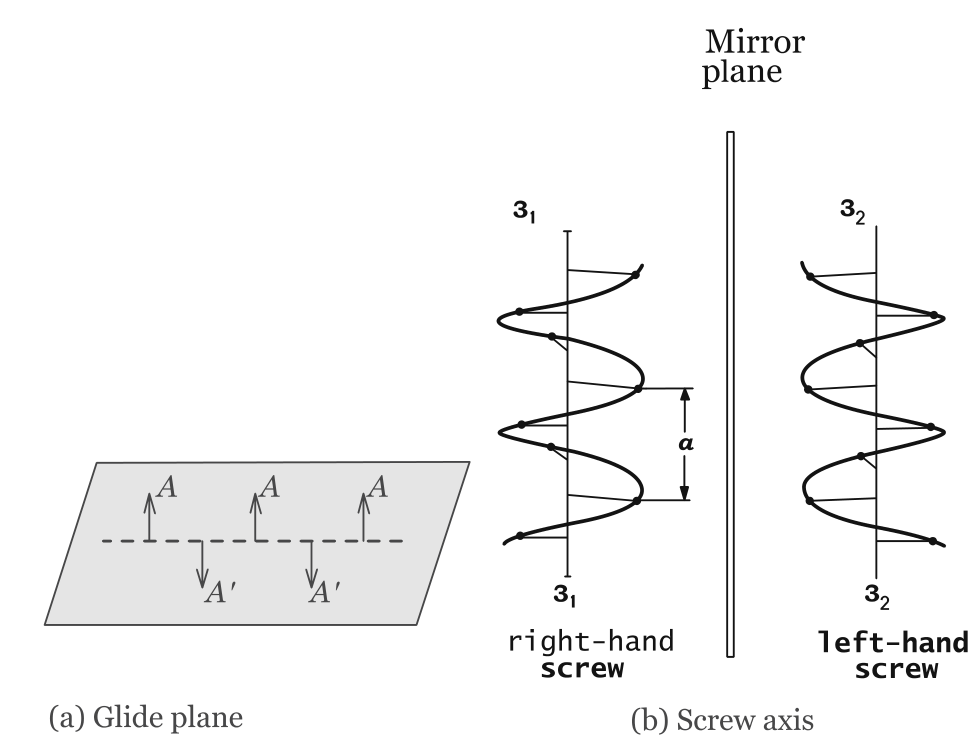
\includegraphics[width=0.5\linewidth]{fig/glideplane-screwaxis.png}
\caption{(a) The glide plane takes $A$ into $A'$. (b) Right- and left-hand screw axis.}
\label{fig:glideplane-screwaxis}
\end{figure}

Here we are going to study the concept of \textit{space groups}. It is very important to classify the symmetry properties of the system in interest (Twisted Bilayer Graphene). In our examples, we are going to focus on the familiar honeycomb lattice example. The space group is loosely an semi-direct product of the point group and the translation group. Given a fixed lattice, all the linear transformations that carry the lattice into itself belong to the space group. A useful matrix representation for $G$ is:
\begin{equation} \label{eq:spacegroup-rep}
\sg{R_\alpha}{\vtau} =
\begin{pmatrix}
1 & 0 \\
\vtau & R_\alpha
\end{pmatrix},
\end{equation}
where $0$ is a row of three zeros, $\vtau$ is a column vector and $R_\alpha$ is $3\times 3$ rotation matrix.

The inverse of an element is given by
\begin{equation} \label{eq:inv-spacegroup}
\sg{R_\alpha}{\vtau}^{-1} =
\begin{pmatrix}
1 & 0 \\
-R_\alpha^{-1}\vtau & R_\alpha^{-1}
\end{pmatrix} =
\sg{R_\alpha^{-1}}{-R_\alpha^{-1}\vtau}.
\end{equation}

Let's take the honeycomb lattice as the example. The space group of interest $P622$ \cite{thesis_rennella} is symmorphic (Table 9.1 of \cite{dresselhaus}). Therefore it is impossible to find a screw axis or glide plane. We have to rely on pure translation + pure point group.

\textbf{IT IS MUCH BETTER TO MAKE THE EXAMPLE 2x2}

For example, let's take a translation of $d(\cos30^\circ, \sin30^\circ)$ with a rotation of $60^\circ$. The result is
$$
R_{\mathcal{E}} =
\begin{pmatrix}
\frac{1}{2} & -\frac{\sqrt{3}}{2} \\
\frac{\sqrt{3}}{2} & \frac{1}{2} \\
\end{pmatrix}
$$

Consider the two basis $\mathcal{E} = \{\ihat, \jhat\}$, and $\mathcal{B} = \{\v_1, \v_2\}$, where $\v_1 = a \ihat$, and $\v_2 = a \qty(\frac{1}{2}\ihat + \frac{\sqrt{3}}{2} \jhat)$. The change of basis matrix is from $\mathcal{B}$ to $\mathcal{E}$ is $M_{\mathcal{B}\to\mathcal{E}}$ and its inverse is $M_{\mathcal{E}\to\mathcal{B}} = M_{\mathcal{B}\to\mathcal{E}}^{-1}$
$$
M_{\mathcal{B} \to \mathcal{E}} =
a
\begin{pmatrix}
1 & \frac{1}{2} \\
0 & \frac{\sqrt{3}}{2}
\end{pmatrix},
\quad
M_{\mathcal{E} \to \mathcal{B}} = M_{\mathcal{B}\to\mathcal{E}}^{-1} =
\frac{1}{a}
\begin{pmatrix}
1 & -\frac{1}{\sqrt{3}} \\
0 & \frac{2}{\sqrt{3}}
\end{pmatrix},
$$

In this basis, the rotation matrix becomes
$$
R_{\mathcal{B}} =  M_{\mathcal{E} \to \mathcal{B}} \, R_{\mathcal{E}} \, M_{\mathcal{B}\to\mathcal{E}} =
\begin{pmatrix}
0 & -1 \\
1 &  0
\end{pmatrix}
$$

The translation of $d(\cos 30^\circ, \sin 30^\circ)$ is
$$
\bm{\tau}_E = a \begin{pmatrix} \frac{1}{2} \\ \frac{\sqrt{3}}{6} \end{pmatrix} \implies
\bm{\tau}_B = M_{\mathcal{E} \to \mathcal{B}} \bm{\tau}_E =
\begin{pmatrix}
\frac{1}{3} \\ \frac{1}{3}
\end{pmatrix}.
$$

Our space group matrix (in the $\mathcal{B}$ basis) is
$$
\{R_{\mathcal{B}}, \vtau_{\mathcal{B}}\} =
\begin{pmatrix}
1 & 0 & 0 \\
1/3 & 0 & -1 \\
1/3 & 1 & 0 \\
\end{pmatrix}
$$

Some arbitrary lattice vector is represented by $\u_s = m \v_1 + n\v_2 + \bm{\beta_s}$, where $s = A, B$ represents the sublattice index, with $\bm{\beta}_A = \0$, $\bm{\beta}_B = \vtau_{\mathcal{B}}$. We have
$$
\{R_{\mathcal{B}}, \vtau_{\mathcal{B}}\} \, \u_A =
\begin{pmatrix}
1 & 0 & 0 \\
1/3 & 0 & -1 \\
1/3 & 1 & 0 \\
\end{pmatrix}
\begin{pmatrix}
1 \\ m \\ n
\end{pmatrix}
=
$$
$$
=
\begin{pmatrix}
1 \\ -n + \frac{1}{3} \\ m+n+\frac{1}{3}
\end{pmatrix}
=
\begin{pmatrix}
1 \\ -n \v_1 + (m+n) \v_2 + \vtau_{\mathcal{B}}
\end{pmatrix}
\in B.
$$

$$
\{R_{\mathcal{B}}, \vtau_{\mathcal{B}}\} \, \u_B =
\begin{pmatrix}
1 & 0 & 0 \\
1/3 & 0 & -1 \\
1/3 & 1 & 0 \\
\end{pmatrix}
\begin{pmatrix}
1 \\ m + \frac{1}{3} \\ n + \frac{1}{3}
\end{pmatrix}
=
$$
$$
=
\begin{pmatrix}
1 \\ -n \\ 1+m+n
\end{pmatrix}
=
\begin{pmatrix}
1 \\ -n \v_1 + (1+m+n) \v_2
\end{pmatrix}
\in A.
$$

Therefore, the lattice is invariant by the space group operation $\{R_{\mathcal{B}}, \vtau_{\mathcal{B}}\}$.

\n

\textbf{Example of nonsymmorphic space group}: Tellurium screw axis $3_1$ (achei figura na internet). Glide plane triangular lattice (gerar minha própria figura), translation $a/2$ and reflection. There is also this link \href{https://physics.stackexchange.com/questions/568476/example-of-a-space-group-which-does-not-contain-the-point-group-as-a-subgroup}{here} which explains the glide plane symmetry in Kagomé lattice. \textbf{Maybe it is better to consider the H2O ice hexagonal.}

%\section{Site-symmetry group}
%
%Let $G$ be a space group associated with its corresponding lattice and a choice of origin. The subgroup of all symmetry operations of $G$ that leaves a point $P$ of the real space inveriant is called the \textit{site-symmetry group} of $P$. This point $P$ is called \textit{of special position} with respect to $G$ if there is at least one non-trivial (not the identity) symmetry operation of $G$ that leaves $P$ invariant.
%
%For a general operation $g$ of $G$, the point $P$ will be mapped into some other point $Q = g P$. If $P$ is of special position with site-symmetry group $G_P$, then $Q$ will also be of special position and its site-symmetry group $G_Q$ will be a conjugate group of $G_P$, namely $G_Q = g G_P g^{-1}$. In fact, we have
%$$
%G_Q Q = g G_P g^{-1} Q = g G_P P = g P = Q.
%$$
%
%If we apply of all operations of $G$ to $P$, we obtain the \textit{crystallographic orbit} of $P$, which is the set of points $Q$ with site-symmetry groups conjugate to $G_P$. If $P$ is of special position, we call its crystallographic orbit a \textit{Wyckoff position} of the space group $G$. Therefore, the concept of Wyckoff position refers to a \textbf{set of points of special position with site-symmetry groups conjugates of each other}.

%%%%%%%%%%%%%%%%%%%%%%%%%%%%%%%%%%%%%%%%%%%%%%%%%%%%%%%%%%%%%%%%%%%%%%%%%%%%%%%%%%%%%%%%%%%%%%%%%%
\subsection{Translation subgroup}
%%%%%%%%%%%%%%%%%%%%%%%%%%%%%%%%%%%%%%%%%%%%%%%%%%%%%%%%%%%%%%%%%%%%%%%%%%%%%%%%%%%%%%%%%%%%%%%%%%

All the elements $\sg{\eps}{\tau}$ of the the space group $G$ constitute the translation group $T$. It is a subgroup of $G$ and defines the Bravais lattice. More than that, $T$ is a normal subgroup of $G$, which means that $g T g^{-1} = T$ for every $g \in G$. Because of that, the cosets
$$
\{ \sg{R_\alpha}{\tau'} \sg{\eps}{\tau} \mid \sg{\eps}{\tau} \in T \} \in G/T
$$
form a factor group of the space group $G$.

This factor group $G/T$ is actually isomorphic to the point group of $G$.

%%%%%%%%%%%%%%%%%%%%%%%%%%%%%%%%%%%%%%%%%%%%%%%%%%%%%%%%%%%%%%%%%%%%%%%%%%%%%%%%%%%%%%%%%%%%%%%%%%
\subsection{Symmorphic and Nonsymmorphic Space Groups} \label{sec:symmorphic_groups}
%%%%%%%%%%%%%%%%%%%%%%%%%%%%%%%%%%%%%%%%%%%%%%%%%%%%%%%%%%%%%%%%%%%%%%%%%%%%%%%%%%%%%%%%%%%%%%%%%%

In a space group $G$, we can always rewrite its elements in the form
$$
\sg{R_\alpha}{\tau} = \sg{R_\alpha}{r_n + \tau} = \sg{\eps}{r_n} \sg{R_\alpha}{\tau_\alpha},
$$
where $r_n$ is a general vector of the Bravais lattice and $\tau_\alpha$ is either zero or a non-primitive Bravais lattice translation. Basically, we will have $\tau_\alpha = 0$ for simple group operations and $\tau_\alpha \neq 0$ for glide planes or screw axis.

If, with a suitable choice of origin, all the elements of $G$ can be written in the form $\sg{R_\alpha}{\tau} = \sg{R_\alpha}{r_n} = \sg{\eps}{r_n} \sg{R_\alpha}{0}$ ($\tau_\alpha = 0$ for every symmetry operation), then call $G$ a \textit{symmorphic} space group.


%%%%%%%%%%%%%%%%%%%%%%%%%%%%%%%%%%%%%%%%%%%%%%%%%%%%%%%%%%%%%%%%%%%%%%%%%%%%%%%%%%%%%%%%%%%%%%%%%%%
%\section{Space groups in Reciprocal Space}
%%%%%%%%%%%%%%%%%%%%%%%%%%%%%%%%%%%%%%%%%%%%%%%%%%%%%%%%%%%%%%%%%%%%%%%%%%%%%%%%%%%%%%%%%%%%%%%%%%%
%
%%%%%%%%%%%%%%%%%%%%%%%%%%%%%%%%%%%%%%%%%%%%%%%%%%%%%%%%%%%%%%%%%%%%%%%%%%%%%%%%%%%%%%%%%%%%%%%%%%%
%\subsection{Group of the wave vector $G_{\k}$ and the Star of $\k$}
%%%%%%%%%%%%%%%%%%%%%%%%%%%%%%%%%%%%%%%%%%%%%%%%%%%%%%%%%%%%%%%%%%%%%%%%%%%%%%%%%%%%%%%%%%%%%%%%%%%
%
%If we have
%$$
%(\hat{P}_\alpha \R_n) \vdot \K_m = 2 \pi N,
%$$
%than
%$$
%\R_n \vdot (\hat{P}_\alpha^{-1} \K_m) = 2 \pi N.
%$$
%
%Thus, the effect of an operator $\hat{P}_\alpha$ on a direct lattice vector $\R_n$ is equivalent to the effect of the operator $\hat{P}_\alpha^{-1}$ on the corresponding reciprocal lattice vector $\K_m$.
%
%\n
%
%The group of the wave vector is formed by the set of space group operations which transform $\k$ into itself, or into an equivalent $\k = \k + \K_m$, where $\K_m$ is a vector of the reciprocal lattice.
%
%All the symmetry operation of the space group $G$ take the point $\k = 0$ into an equivalent point, so that the group of the wave vector at $\k = 0$ corresponds to $G$. Furthermore, the $G_\k$ for $\k \neq 0$ remains a subgroup of $G$.
%
%\n
%
%The set of wave vectors $\k'$ which are obtained by carrying out all the point group operations on $\k$ is called \textit{star of} $\k$.
%
%\n
%
%In summary
%$$
%\text{real space} \iff \text{reciprocal space}
%$$
%$$
%\text{site-symmetry group} \iff \text{group of wave vector }G_\k
%$$
%$$
%\text{Wyckoff position} \iff \text{star of }\k
%$$

\section{Magnetic Space Groups} \label{sec:magnetic_space_groups}

Magnetic moments in a solid appears when there are unpaired electrons in electronic shells. A common example is the Hund's rule, which favours the ``ferromagnetic'' interaction so that an intrinsic magnetic moment appears. Below the ordering temperature, a magnetic structure is formed, and above the ordering temperature, the system is in the paramagnetic state.

In this section, we are going to introduce the concept of magnetic space group (Shubnikov group), which is important to study magnetic structures. But our main interest is to apply its theory to analyze symmetries of the TBG system, which has negligible SOC and we can say ``it is spinless'', but we can use the same formalism on the sublattice degree of freedom.

To study the symmetries of magnetic configurations, we introduce the time reversal operator, denoted by $T$ or $1'$. In the context of magnetic systems, this operator acts on magnetic moments that are ``classical axial vectors''. Its action consists of reverting the sense of the current loop, so that the orientation of the magnetic moment is reversed.

\begin{figure}[H]
\centering
\begin{subfigure}{.4\textwidth}
  \centering
  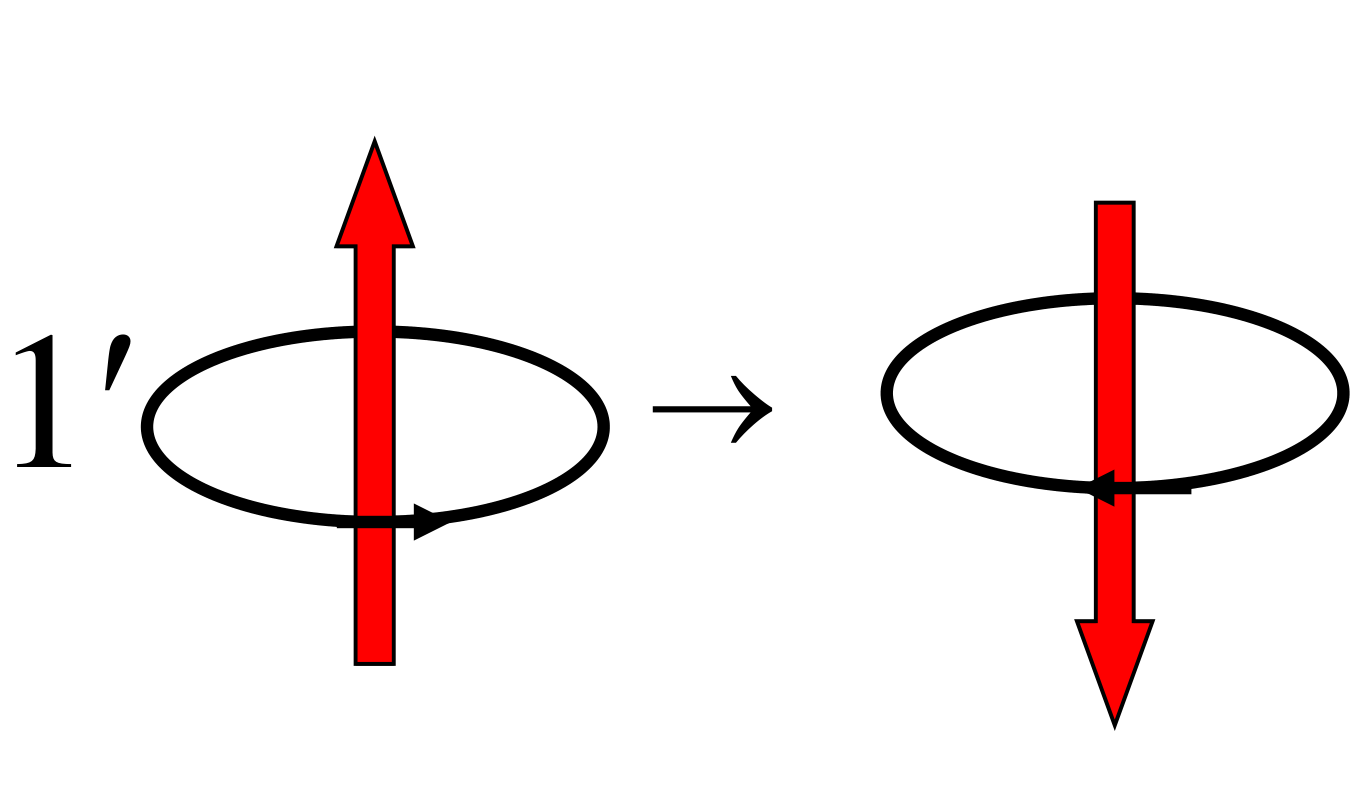
\includegraphics[height=0.4\linewidth]{fig/timerev.png}
  \caption{}
  \label{fig:timerev}
\end{subfigure}%
\begin{subfigure}{.6\textwidth}
  \centering
  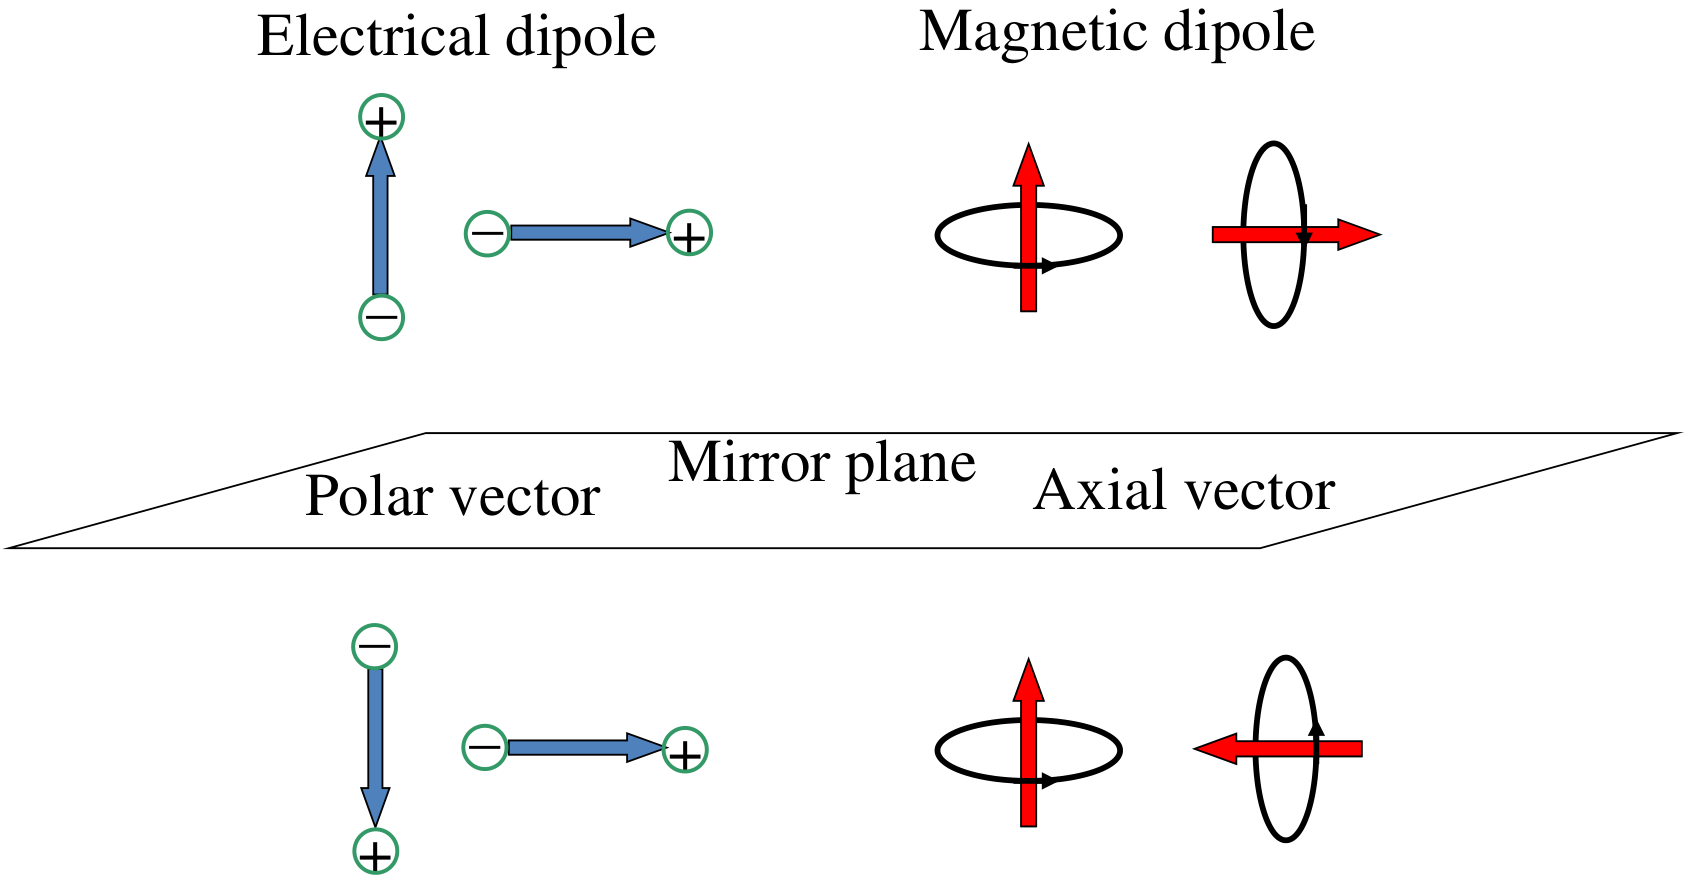
\includegraphics[width=\linewidth]{fig/axialvec.png}
  \caption{}
  \label{fig:axialvec}
\end{subfigure}
\caption{.}
\label{fig:geometry}
\end{figure}

We define the time reversal group formed by only two elements $R = \{1, 1'\}$. Any magnetic group $M$ can be obtained as a subgroup of the direct product of $R$ with another group $G$, such that $M \leq G \otimes R$. The group $G \otimes \{1\}$ is a magnetic group, called ``colourless''. The paramagnetic (``grey'') groups are of the form $P = G \cup G1'$. The other form to construct magnetic groups (``black-white'') is
$$
M = H + (G - H) 1',
$$
where $H \leq G$ is a subgroup of index 2.


\section{Application to TBG} \label{sec:application_to_tbg}

The magnetic point group of the BM model of TBG is $6'2'2$ in Hermann-Mauguin notation. According to the notation, we can choose its generators to be $C_{6z} T$, $C_{2y} T$ and $C_{2x}$.

\begin{figure}[H]
\centering
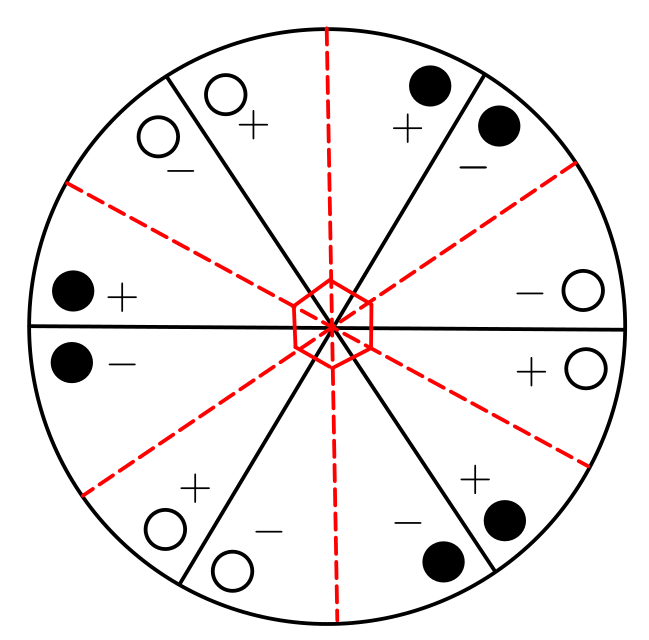
\includegraphics[width=0.5\linewidth]{fig/622_magnetic.png}
\caption{Representation of the magnetic point group $6'2'2$.}
\label{fig:622_magnetic}
\end{figure}





%%%%%%%%%%%%%%%%%%%%%%%%%%%%%%%%%%%%%%%%%%%%%%%%%%%%%%%%%%%%%%%%%%%%%%%%%%%%%%%%%%%%%%%%%%%%%%%%%%
%%%%%%%%%%%%%%%%%%%%%%%%%%%%%%%%%%%%%%%%%%%%%%%%%%%%%%%%%%%%%%%%%%%%%%%%%%%%%%%%%%%%%%%%%%%%%%%%%%


%%%%%%%%%%%%%%%%%%%%%%%%%%%%%%%% COMMENT THIS TO COMPILE main.tex %%%%%%%%%%%%%%%%%%%%%%%%%%%%%%%%
%%-----
%% Referências bibliográficas
%%-----
\addcontentsline{toc}{chapter}{\bibname}
%\bibliographystyle{abntex2-num}
\bibliography{citations}
\bibliographystyle{ieeetr}
\end{document}
%%%%%%%%%%%%%%%%%%%%%%%%%%%%%%%% COMMENT THIS TO COMPILE main.tex %%%%%%%%%%%%%%%%%%%%%%%%%%%%%%%%
